\documentclass{article}

  % packages
    % basic stuff for rendering math
    \usepackage[letterpaper, top=1in, bottom=1in, left=1in, right=1in]{geometry}
    \usepackage[utf8]{inputenc}
    \usepackage[english]{babel}
    \usepackage{amsmath} 
    \usepackage{amssymb}
    \usepackage{natbib}

    % extra math symbols and utilities
    \usepackage{mathtools}        % for extra stuff like \coloneqq
    \usepackage{mathrsfs}         % for extra stuff like \mathsrc{}
    \usepackage{centernot}        % for the centernot arrow 
    \usepackage{bm}               % for better boldsymbol/mathbf 
    \usepackage{bbm}              % for indicator functions
    \usepackage{enumitem}         % better control over enumerate, itemize
    \usepackage{hyperref}         % for hypertext linking
    \usepackage{xr-hyper}
    \usepackage{fancyvrb}         % for better verbatim environments
    \usepackage{newverbs}         % for texttt{}
    \usepackage{xcolor}           % for colored text 
    \usepackage{listings}         % to include code
    \usepackage{lstautogobble}    % helper package for code
    \usepackage{parcolumns}       % for side by side columns for two column code
    \usepackage{algorithm}
    \usepackage{algpseudocode}

    % page layout
    \usepackage{fancyhdr}         % for headers and footers 
    \usepackage{uniquecounter} 
    \usepackage{lastpage}         % to include last page number in footer 
    \usepackage{parskip}          % for no indentation and space between paragraphs    
    \usepackage[T1]{fontenc}      % to include \textbackslash
    \usepackage{footnote}
    \usepackage{etoolbox}

    % for custom environments
    \usepackage{tcolorbox}        % for better colored boxes in custom environments
    \tcbuselibrary{breakable}     % to allow tcolorboxes to break across pages

    % figures
    \usepackage{pgfplots}
    \pgfplotsset{compat=1.18}
    \usepackage{float}            % for [H] figure placement
    \usepackage{tikz}
    \usepackage{tikz-cd}
    \usepackage{circuitikz}
    \usetikzlibrary{positioning, shapes, arrows, fit, calc}
    \usepackage{graphicx}
    \usepackage{caption} 
    \usepackage{subcaption}
    \captionsetup{font=small}

    % for tabular stuff 
    \usepackage{dcolumn}

    \usepackage[nottoc]{tocbibind}
    \pdfsuppresswarningpagegroup=1
    \hfuzz=5.002pt                % ignore overfull hbox badness warnings below this limit

  % New and replaced operators
    \DeclareMathOperator{\Tr}{Tr}
    \DeclareMathOperator{\Sym}{Sym}
    \DeclareMathOperator{\Span}{span}
    \DeclareMathOperator{\elbo}{ELBO}
    \DeclareMathOperator{\std}{std}
    \DeclareMathOperator{\Cov}{Cov}
    \DeclareMathOperator{\Var}{Var}
    \DeclareMathOperator{\proj}{proj}
    \DeclareMathOperator{\Corr}{Corr}
    \DeclareMathOperator{\pos}{pos}
    \DeclareMathOperator*{\argmin}{\arg\!\min}
    \DeclareMathOperator*{\argmax}{\arg\!\max}
    \newcommand{\ket}[1]{\ensuremath{\left|#1\right\rangle}}
    \newcommand{\bra}[1]{\ensuremath{\left\langle#1\right|}}
    \newcommand{\braket}[2]{\langle #1 | #2 \rangle}
    \newcommand{\qed}{\hfill$\blacksquare$}     % I like QED squares to be black 

  % Custom Environments
    \newtcolorbox[auto counter, number within=section]{question}[1][]
    {
      colframe = orange!25,
      colback  = orange!10,
      coltitle = orange!20!black,  
      breakable, 
      title = \textbf{Question \thetcbcounter ~(#1)}
    }

    \newtcolorbox[auto counter, number within=section]{exercise}[1][]
    {
      colframe = teal!25,
      colback  = teal!10,
      coltitle = teal!20!black,  
      breakable, 
      title = \textbf{Exercise \thetcbcounter ~(#1)}
    }
    \newtcolorbox[auto counter, number within=section]{solution}[1][]
    {
      colframe = violet!25,
      colback  = violet!10,
      coltitle = violet!20!black,  
      breakable, 
      title = \textbf{Solution \thetcbcounter}
    }
    \newtcolorbox[auto counter, number within=section]{lemma}[1][]
    {
      colframe = red!25,
      colback  = red!10,
      coltitle = red!20!black,  
      breakable, 
      title = \textbf{Lemma \thetcbcounter ~(#1)}
    }
    \newtcolorbox[auto counter, number within=section]{theorem}[1][]
    {
      colframe = red!25,
      colback  = red!10,
      coltitle = red!20!black,  
      breakable, 
      title = \textbf{Theorem \thetcbcounter ~(#1)}
    } 
    \newtcolorbox[auto counter, number within=section]{proposition}[1][]
    {
      colframe = red!25,
      colback  = red!10,
      coltitle = red!20!black,  
      breakable, 
      title = \textbf{Proposition \thetcbcounter ~(#1)}
    } 
    \newtcolorbox[auto counter, number within=section]{corollary}[1][]
    {
      colframe = red!25,
      colback  = red!10,
      coltitle = red!20!black,  
      breakable, 
      title = \textbf{Corollary \thetcbcounter ~(#1)}
    } 
    \newtcolorbox[auto counter, number within=section]{proof}[1][]
    {
      colframe = orange!25,
      colback  = orange!10,
      coltitle = orange!20!black,  
      breakable, 
      title = \textbf{Proof. }
    } 
    \newtcolorbox[auto counter, number within=section]{definition}[1][]
    {
      colframe = yellow!25,
      colback  = yellow!10,
      coltitle = yellow!20!black,  
      breakable, 
      title = \textbf{Definition \thetcbcounter ~(#1)}
    } 
    \newtcolorbox[auto counter, number within=section]{example}[1][]
    {
      colframe = blue!25,
      colback  = blue!10,
      coltitle = blue!20!black,  
      breakable, 
      title = \textbf{Example \thetcbcounter ~(#1)}
    } 
    \newtcolorbox[auto counter, number within=section]{code}[1][]
    {
      colframe = green!25,
      colback  = green!10,
      coltitle = green!20!black,  
      breakable, 
      title = \textbf{Code \thetcbcounter ~(#1)}
    } 
    \newtcolorbox[auto counter, number within=section]{algo}[1][]
    {
      colframe = green!25,
      colback  = green!10,
      coltitle = green!20!black,  
      breakable, 
      title = \textbf{Algorithm \thetcbcounter ~(#1)}
    } 
    
    \definecolor{dkgreen}{rgb}{0,0.6,0}
    \definecolor{gray}{rgb}{0.5,0.5,0.5}
    \definecolor{mauve}{rgb}{0.58,0,0.82}
    \definecolor{darkblue}{rgb}{0,0,139}
    \definecolor{lightgray}{gray}{0.93}
    \renewcommand{\algorithmiccomment}[1]{\hfill$\triangleright$\textcolor{blue}{#1}}

    % default options for listings (for code)
    \lstset{
      autogobble,
      frame=ltbr,
      language=Python,                           % the language of the code
      aboveskip=3mm,
      belowskip=3mm,
      showstringspaces=false,
      columns=fullflexible,
      keepspaces=true,
      basicstyle={\small\ttfamily},
      numbers=left,
      firstnumber=1,                        % start line number at 1
      numberstyle=\tiny\color{gray},
      keywordstyle=\color{blue},
      commentstyle=\color{dkgreen},
      stringstyle=\color{mauve},
      backgroundcolor=\color{lightgray}, 
      breaklines=true,                      % break lines
      breakatwhitespace=true,
      tabsize=3, 
      xleftmargin=2em, 
      framexleftmargin=1.5em, 
      stepnumber=1
    }

  % Page style
    \pagestyle{fancy}
    \fancyhead[L]{Kernels and Smoothers}
    \fancyhead[C]{Muchang Bahng}
    \fancyhead[R]{Spring 2024} 
    \fancyfoot[C]{\thepage / \pageref{LastPage}}
    \renewcommand{\footrulewidth}{0.4pt}          % the footer line should be 0.4pt wide
    \renewcommand{\thispagestyle}[1]{}  % needed to include headers in title page

\begin{document}

\title{Kernels and Smoothers}
\author{Muchang Bahng}
\date{Spring 2025}

\maketitle
\tableofcontents
\pagebreak

This covers computability theory, complexity theory, and automata theory. 
Alphabet. Boolean logic


\section{Smoothers} 

\subsection{Linear Smoothers} 

\section{K Nearest Neighbors} 

  KNN was first introduced by Cover in 1967 \cite{1967cover}. 

\subsection{Classification}

  \begin{question}[To Do]
    Maybe similar like a kernel regression?  
  \end{question}

  Given a bunch of points in a metric space $(\mathcal{X}, d)$ that have classification labels, we want to label new datapoints $\hat{\mathbf{x}}$ based on the labels of other points that already exist in our dataset. One way to look at it is to look for close points within the dataset and use their labels to predict the new ones. 

  \begin{definition}[Closest Neighborhood]
    Given a dataset $\mathcal{D} = \{\mathbf{x}^{(i)}, \mathbf{y}^{(i)}\}$ and a point $\hat{\mathbf{x}} \in (\mathcal{X}, d)$, let the \textbf{k closest neighborhood} of $\hat{\mathbf{x}}$ be $N_k (\hat{\mathbf{x}}) \subset [N]$ defined as the indices $i$ of the $k$ points in $\mathcal{D}$ that is closest to $\hat{\mathbf{x}}$ with respect to the distance metric $d_\mathcal{X}$. 
  \end{definition}

  \begin{definition}[K Nearest Neighbors]
    The \textbf{K Nearest Neighbors (KNN)} is a discriminative nonparametric supervised learning algorithm that doesn't have a training phase. Given a new point $\hat{\mathbf{x}}$, we look at all points in its k closest neighborhood, and $h(\hat{\mathbf{x}})$ will be equal to whatever the majority class will be in. Let us one-hot encode the labels $\mathbf{y}^{(i)}$ into $\mathbf{e}_i$'s, and the number of data point in the $i$th class can be stored in the variable 
    \begin{equation}
      a_i = \sum_{i \in N_k (\hat{\mathbf{x}})} 1_{\{\mathbf{y}^{(i)} = \mathbf{e}_i\}}
    \end{equation}
    which results in the vector storing the counts of labels in the k closest neighborhood 
    \begin{equation}
      \mathbf{a} = (a_1, a_2, \ldots, a_\mathcal{K}) = \bigg( \sum_{i \in N_k (\hat{\mathbf{x}})} 1_{\{\mathbf{y}^{(i)} = \mathbf{e}_1\}}, \sum_{i \in N_k (\hat{\mathbf{x}})} 1_{\{\mathbf{y}^{(i)} = \mathbf{e}_2\}}, \ldots, \sum_{i \in N_k (\hat{\mathbf{x}})} 1_{\{\mathbf{y}^{(i)} = \mathbf{e}_\mathcal{K}\}} \bigg) 
    \end{equation}
    and take the class with the maximum element as our predicted label. 
  \end{definition}

  The best choice of $K$ depends on the data: 
  \begin{enumerate}
    \item Larger values of $K$ reduces the effect of noise on the classification, but make boundaries between classes less distinct. The number of misclassified data points (error) increases. 
    \item Smaller values are more sensitive to noise, but boundaries are more distinct and the number of misclassified data points (error) decreases.
  \end{enumerate}
  Too large of a $K$ value may increase the error too much and lead to less distinction in classification, while too small of a k value may result in us overclassifying the data. Finally, in binary (two class) classification problems, it is helpful to choose $K$ to be odd to avoid tied votes.

  This is an extremely simple algorithm that may not be robust. For example, consider $K \geq 3$, and we are trying to label a point $\hat{\mathbf{x}}$ that happens to be exactly where one point is on our dataset $\mathbf{x}^{(i)}$. Then, we should do $h(\hat{\mathbf{x}}) = y^{(i)}$, but this may not be the case if there are no other points with class $y^{(i)}$ in the k closest neighborhood of $\mathbf{x}^{(i)}$. Therefore, we want to take into account the distance of our new points from the others. 

  \begin{definition}[Weighted Nearest Neighbor Classifier]
    Let us define a monotinically decreasing function $\omega: \mathbb{R}_0^+ \mapsto \mathbb{R}_0^+$. Given a point $i \in N_k (\hat{\mathbf{x}})$, we can construct the weight of our matching label as inversely proportional to the distance: $\omega_i [ d(\hat{\mathbf{x}}, \mathbf{x}^{(i)})]$ and store them as 
    \begin{equation}
      \mathbf{a} = (a_1, a_2, \ldots, a_\mathcal{K}) = \bigg( \sum_{i \in N_k (\hat{\mathbf{x}})} \omega_i 1_{\{\mathbf{y}^{(i)} = \mathbf{e}_1\}}, \sum_{i \in N_k (\hat{\mathbf{x}})} \omega_i 1_{\{\mathbf{y}^{(i)} = \mathbf{e}_2\}}, \ldots, \sum_{i \in N_k (\hat{\mathbf{x}})} \omega_i 1_{\{\mathbf{y}^{(i)} = \mathbf{e}_\mathcal{K}\}} \bigg)
    \end{equation}
    and again take the class with the maximum element. 
  \end{definition}

  One caveat of KNN is in high dimensional spaces, as its performance degrades quite badly due to the curse of dimensionality. 

  \begin{example}[Curse of Dimensionality in KNN]
    Consider a dataset of $N$ samples uniformly distributed in a $d$-dimensional hypercube. Now given a point $x \in [0, 1]^d$, we want to derive the expected radius $r_k$ required to encompass its $k$ nearest neighbors. Let us define this ball to be $B_{r_k} \coloneqq \{ z \in \mathbb{R}^d \mid ||z - x ||_2 \leq r_k \}$. Since thse $N$ points are uniformly distributed, the expected number of points contained in $B_{r_k} (x)$ is simply the proportion of the volume that $B_{r_k} (x)$ encapsulates in the box, multiplied by $N$. Therefore, for some fixed $x$ and $r$, let us denote $Y(x, y)$ as the random variable representing the number of points contained within $B_r (x)$. By linearity of expectation and summing over the expectation for whether each point will be in the ball, we have 
    \[\mathbb{E}[Y (x, r)] = N \cdot \frac{\mu(B_r (x) \cap [0, 1]^d) }{\mu([0, 1]^d)}\]
    where $\mu$ is the Lebesgue measure of $\mathbb{R}^d$. Let us assume for not that we don't need to worry about cases where the ball is not fully contained within the cube, so we can just assume that $Y$ is only dependent on $r$: $Y(r)$. Also, since the volume of the hypercube is $1$,  $\mu([0, 1]^d) = 1$ and we get 
    \[\mathbb{E}[Y(r)] = N \cdot C_d \cdot r^d\]
    which we set equal to $k$ and evaluate for $r$. $C_d$ is a constant such that the volume of the hypersphere of radius $r$ can be derived as $V = C_d \cdot r^d$. We therefore get 
    \[N \cdot C_d \cdot r_k^d = k \implies r_k = \bigg( \frac{k}{N C_d} \bigg)^{1/d}\]
    It turns out that $C_d$ decreases exponentially, so the radius $r_k$ explodes as $d$ grows. Another way of looking at this is that in high dimensions, the $\ell_2$ distance between all the pairwise points are close in every single dimension, so it becomes harder to distinguish points that are close vs those that are far.  
  \end{example} 

  \subsection{Approximate K Nearest Neighbors}

\subsection{Regression}

  When we want to do nonparametric regression, i.e. when dealing with nonlinear functions, we can construct a function that uses local averaging of its nearby points. 

  \begin{example}[Local Averaging]
    Say that we want to fit some function through a series of datapoints in simple regression (one covariate). Then, what we can do is take some sliding window and our vale of the function at a point $x$ is the average of all values in the window $[x - \delta, x + \delta]$. 
    \begin{figure}[H]
      \centering 
      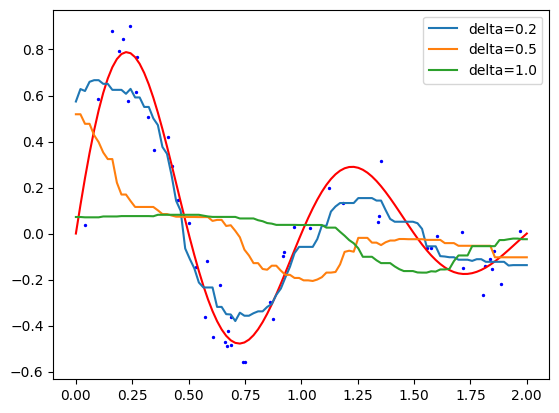
\includegraphics[scale=0.6]{img/kmeans_smoother.png}
      \caption{K means smoother} 
      \label{fig:kmeans_smoother}
    \end{figure}
  \end{example}

  \begin{code}[MWS of K Nearest Neighbor Regression in scikit-learn]
    Local averaging is implemented as the K nearest neighbor regressor in scikit learn. It is slightly different in the way that it doesn't use the points within a certain $\delta$ away but rather the $K$ nearest points. Either way, a minimal working example of this is 
    \begin{lstlisting}
      X = [[0], [1], [2], [3]]
      y = [0, 0, 1, 1]
      from sklearn.neighbors import KNeighborsRegressor
      neigh = KNeighborsRegressor(n_neighbors=2)
      neigh.fit(X, y)
      print(neigh.predict([[1.5]])) 
    \end{lstlisting}
  \end{code}

  Note that since $\hat{f}$ is a combination of step functions, this makes it discontinuous at points. 


\section{Kernel Regression and Linear Smoothers} 

  K nearest neighbor regression puts equal weights on both near and far points, as long as they are in the window. This may not be ideal, so a simple modification is to \textit{weigh} these points according to their distance from the middle $x$. We can do this with a kernel, as the name suggests. Now this is not the same thing as a Mercer kernel in RKHS, so to distinguish that I will call it a \textit{local averaging kernel}. 

  \begin{definition}[Local Averaging Kernel]
    A \textbf{kernel} is any smooth, symmetric, and non-negative function $K : \mathbb{R} \to \mathbb{R}$.  
  \end{definition}

  \begin{definition}[Kernel Regression]
    Given some datapoints, $X$, our fitted regressor is of form 
    \begin{equation}
      \hat{f} (X) = \frac{\sum_{i} Y_i K \bigg( \frac{||X - X_i||}{h} \bigg)}{\sum_{i} K \bigg( \frac{||X - X_i||}{h} \bigg)}
    \end{equation}
    where $h$ is the \textbf{bandwidth} and the denominator is made sure so that the coefficients sum to $1$. To get a clearer picture, we are really taking the weighted average of the $Y_i$'s. 
    \begin{equation}
      \hat{f} (X) = \sum_{i} Y_i \ell_i (X) \text{ where } \sum_{i} \ell_i (X) = 1
    \end{equation}
    Denoting $Y = (Y_1, \ldots, Y_n) \in \mathbb{R}^n$ and the vector $f(X) = (f(X_1), \ldots, f(X_n))$, if we can write the kernel function as $\hat{Y} = \hat{f}(X) = S Y$, which in matrix form, is 
    \begin{equation}
      \begin{bmatrix} \hat{Y}_1 \\ \vdots \\ \hat{Y}_n \end{bmatrix} = \begin{bmatrix} \hat{f}(X_1) \\ \vdots \\ \hat{f} (X_n) \end{bmatrix} = \begin{bmatrix} \ell_1 (X_1) & \cdots & \ell_n (X_1) \\ \vdots & \ddots & \vdots \\ \ell_1 (X_n) & \cdots & \ell_n (X_n) \end{bmatrix} \begin{bmatrix} Y_1 \\ \vdots \\ Y_n \end{bmatrix} 
    \end{equation}
    then we say that we have a \textbf{linear smoother}, with stochastic matrix $S$ being our \textbf{smoothing matrix}. 
  \end{definition}

  The reason we'd like to have the weights to sum to $1$ is that if we had data that was constant (i.e. all $Y_i$'s are the same), then the fitted function should be constant at that value as well. Furthermore, the theme of linearity is important and will be recurring. The kernel estimator is defined for all $X$, but it's important to see its behavior at the training points $X_i$. The estimator $\hat{Y} = \hat{f}(X)$ is a linear combination of the $Y_i$'s, and the coefficients $\ell_i (X_j)$ depend on the values of $X_j$. Therefore, we have $\hat{Y} = S Y$, which is very similar to the equation $\hat{Y} = H Y$ in linear regression, where $H$ is the hat matrix that projects $Y$ onto the column space of $X$. Nonparametric regression has the same form, but rather than being a projection, it is a linear smoothing matrix. Therefore, this theme unifies both linear regression and nonparametric regression. Linear smoothers, spline smoother, Gaussian processes, are all just different choices of the smoothing matrix $S$. However, not all nonparametric estimators are linear smoothers, as we will see later. 

  Here are some popular kernels. 

  \begin{definition}[Gaussian Kernel]
    The \textbf{Gaussian kernel} is defined as 
    \begin{equation}
      K(x) = \frac{1}{\sqrt{2 \pi}} e^{-x^2/2}
    \end{equation}
    \begin{figure}[H]
      \centering 
      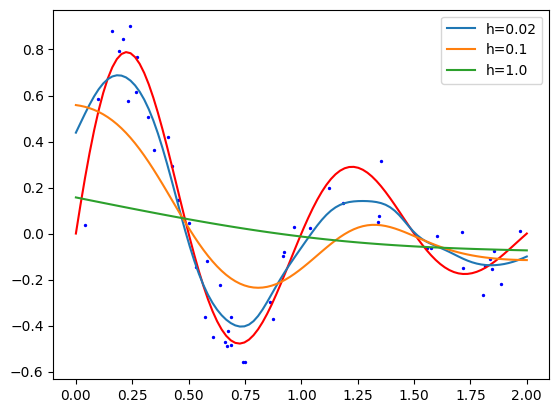
\includegraphics[scale=0.6]{img/gaussian_smoother.png}
      \caption{Gaussian kernel. } 
      \label{fig:gaussian_smoother}
    \end{figure}
  \end{definition}

  \begin{definition}[Box-Car Kernel]
    The \textbf{Box-Car kernel} is defined as 
    \begin{equation}
      K(x) = \frac{1}{2} \mathbbm{1}(|x| \leq 1)
    \end{equation}
    \begin{figure}[H]
      \centering 
      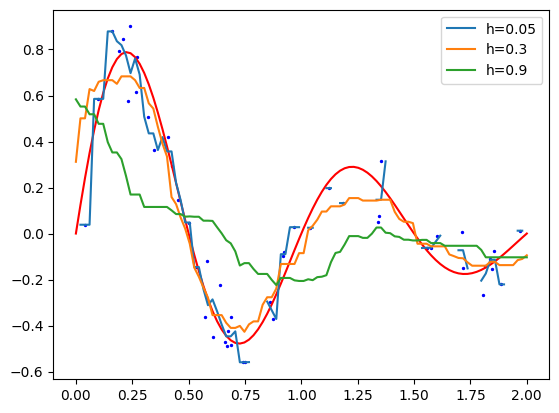
\includegraphics[scale=0.6]{img/boxcar_smoother.png}
      \caption{Boxcar kernel. } 
      \label{fig:boxcar_smoother}
    \end{figure}
  \end{definition}

  \begin{definition}[Epanechnikov Kernel]
    The \textbf{Epanechnikov kernel} is defined as 
    \begin{equation}
      K(x) = \frac{3}{4} (1 - x^2) \mathbbm{1}(|x| \leq 1)
    \end{equation}
    \begin{figure}[H]
      \centering 
      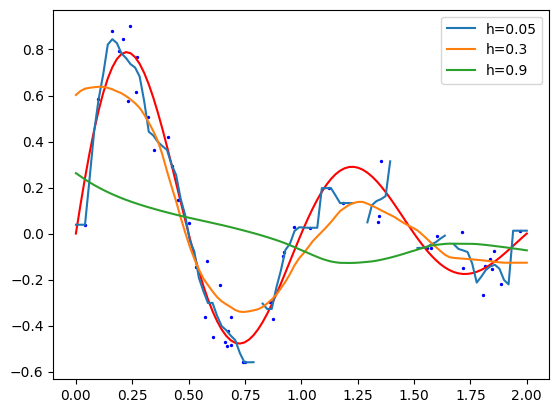
\includegraphics[scale=0.6]{img/epanechnikov_smoother.png}
      \caption{Epanechnikov kernel.} 
      \label{fig:epanechnikov_smoother}
    \end{figure}
  \end{definition}

  It turns out that from a theoretical point of view, the choice of the kernel doesn't really matter. What really matters is the bandwidth $h$ since that is what determines the bias variance tradeoff. To see why, if $h = 0$, then it will simply interpolate the points and variance is extremely high, and if $h = \infty$, then the fitted function will be constant at $\bar{Y}$, leading to high bias. The following theorem formalizes this.  

  \begin{theorem}[Bias Variance Tradeoff of Kernel Regression]
    Suppose that $d = 1$ and that $m^{\prime\prime}$ is bounded. Also suppose that $X$ has a nonzero, differentiable density $p$ and that the support is unbounded. Then, the risk is 
    \begin{align}
      R_n & = \frac{h_n^4}{4} \bigg( \int x^2 K(x) \bigg)^2 \int \bigg( m^{\prime\prime} (x) + 2m^\prime (x) \frac{p^\prime (x)}{p(x)} \bigg)^2 \,dx \\
          & \;\;\; + \frac{\sigma^2 \int K^2(x)\,dx} {n h_n} \int \frac{dx}{p(x)} + o \bigg( \frac{1}{n h_n} \bigg) + o(h_n^4) 
    \end{align}
    The first term is the squared bias and the second term is the variance. 
  \end{theorem}
  \begin{proof}
    We first denote 
    \begin{equation}
      \hat{f}(X) = \frac{\frac{1}{nh} \sum_{i=1}^n K \bigg( \frac{X - X_i}{h} \bigg) Y_i}{\frac{1}{nh} \sum_{i=1}^n K \bigg( \frac{X - X_i}{h} \bigg)} 
    \end{equation}
    where the denominator is the kernel density estimator $\hat{p}(X)$. Therefore, we rewrite
    \begin{align}
      \hat{f} (x) - f(x) & = \frac{\hat{a}(x)}{\hat{p}(x)} - f(x) \\
                         & = \bigg( \frac{\hat{a}(x)}{\hat{p}(x)} - f(x) \bigg) \bigg( \frac{\hat{p}(x)}{p(x) + 1 - \frac{\hat{p}(x)}{p(x)}} \bigg) \\
                         & = \frac{\hat{a}(x) - f(x) \hat{p}(x)}{p(x)} + \frac{(\hat{f}(x) - f(x)) (p(x) - \hat{p}(x))}{p(x)}
    \end{align}
    as $n \rightarrow \infty$ both $\hat{f}(x) - f(x)$ and $p(x) - \hat{p}(x)$ going to $0$, and since they're multiplied in the second term, it will go to $0$ very fast. So the dominant term is the first term, and we can write the above as approximately 
    \begin{equation}
      \hat{f}(x) - f(x) \approx  \frac{\hat{a}(x) - f(x) \hat{p}(x)}{p(x)}
    \end{equation}
    TBD continued. Wasserman lecture 6, 10:00. 
  \end{proof}

  From the theorem above, we can see that if the bandwidth is small, then $h^4$ is small and the bias decreases. However, there is a $h$ term in the denominator of the variance term, which also trades it off. We can furthermore see that the bias is sensitive to $p^\prime / p(x)$. This means that if the density is steep, then the bias will be high. This is known as \textit{design bias}, which is an underlying weakness in smoothing kernel regression. Another problem that is not contained in the theorem is the \textit{boundary bias}, which states that if you're near the boundary of the distribution (i.e. near the boundary of its support), then the bias also explodes. This happens to be very nasty especially in high dimensions where most of the data tends to be near the boundary. It turns out that this can be easily fixed with local polynomial regression, which gets rid of this term in the bias without any cost to variance. This means that this is unnecessary bias. 

  Then you can apply regularization on this to get kernel ridge regression. 

  \begin{code}[MWS of Kernel Ridge Regression in scikit learn]
    \begin{lstlisting}
      from sklearn.kernel_ridge import KernelRidge
      import numpy as np
      n_samples, n_features = 10, 5
      rng = np.random.RandomState(0)
      y = rng.randn(n_samples)
      X = rng.randn(n_samples, n_features)
      krr = KernelRidge(alpha=1.0)
      krr.fit(X, y)
    \end{lstlisting}
  \end{code}


\section{Local Linear/Polynomial Regression}

  Now another way to think about the kernel estimator is as such. Suppose that you're doing linear regression on a bunch of points and you want to choose a $c$ that minimizes the loss. 
  \begin{equation}
    \sum_i (Y_i - c)^2
  \end{equation}

  You would just pick $c = \hat{Y}$. But if you are given some sort of locality condition, that the value of $c$ should depend more on the values closer to it, you're really now minimizing 
  \begin{equation}
    \sum_i (Y_i - c(x))^2 K \bigg( \frac{X_i - x}{h} \bigg)
  \end{equation}

  Minimizing this by setting the derivative equal to $0$ and solving gives us the kernel estimator. Therefore you're fitting some sort of local constant at a point $X$. But why fit a local constant, when you can fit a local line or polynomial? This is the idea behind local polynomial regression.

  \begin{figure}[H]
    \centering 
    \begin{tikzpicture}[scale=1.5]
      % Axes
      \draw[thick] (-2.5,0) -- (2.5,0);
      \draw[thick] (0,-0.5) -- (0,2);

      % X label
      \node[below] at (0.9,-0.3) {$x$};
      \draw[thick, gray, dashed] (0.9,-0.1) -- (0.9,2.1);

      % Gaussian-shaped dotted curve
      \draw[dotted, thick, domain=-2:2, samples=100] plot (\x, {1.2*exp(-0.8*\x*\x) + 0.5});

      % Red linear line
      \draw[red, thick] (0,1.88) -- (1.6,0.53);

      % Blue horizontal line labeled c
      \draw[blue, thick] (0.5,1.1) -- (1.3,1.1);

      % Gaussian curve at bottom
      \draw[thick, domain=0:1.8, samples=100] plot (\x, {0.3*exp(-5*(\x - 0.9)*(\x-0.9))});
    \end{tikzpicture}
    \caption{Rather than using a local constant (blue), we can use a local linear estimator (red).} 
    \label{fig:local_linear_estimator}
  \end{figure}

  Therefore, we can minimize the modified loss. 

  \begin{definition}[Local Polynomial Estimator]
    The \textbf{local polynomial estimator} is a local linear kernel smoother that estimates the function $\hat{f}$ that minimizes the following loss. 
    \begin{equation}
      \argmin_{\beta} \sum_i K \bigg( \frac{X_i - x}{h} \bigg) \big( Y_i - \beta_0 (x) - \beta_1 (x) (x- X_i)\big)
    \end{equation}
  \end{definition}

  So we can fit a line 
  \begin{equation}
    f(\mu) \approx \hat{\beta}_0 (x) + \hat{\beta}_1 (x) (\mu - x)
  \end{equation}
  and simply remove the intercept term to get the local linear estimator. 
  \begin{equation}
    \hat{f}(x) = \hat{\beta}_0 (x)
  \end{equation}
  Note that this is not the same as taking the constant estimate. We are extracting the fitted intercept term and so $\hat{\beta}_0(x) \neq c(x)$. 

\subsection{Weighted Least Squares Solution}

  It turns out that this has an analytic solution. Looking the local polynomial loss should tell you that we're really doing OLS, but weighting the points differently. This sounds a lot like weighted least squares. 

  \begin{theorem}[Weighted Least Squares]
    The solution to the local linear estimator is similar to the weighted least squares solution. 
    \begin{equation}
      \hat{\beta}(x) = \begin{pmatrix} \hat{\beta}_0 (x) \\ \hat{\beta}_1 (x) \end{pmatrix} = (X_x^T W_x X_x)^{-1} X_x^T W_x Y
    \end{equation}
    where we have put the subscript $x$ to emphasize that the matrices are dependent on $x$, and 
    \begin{equation}
      X_x = \begin{pmatrix} 1 & X_1 - x \\ \vdots & \vdots \\ 1 & X_n - x \end{pmatrix} \qquad W_x = \begin{pmatrix} K \big( \frac{X_1 - x}{h} \big) & 0 & \cdots & 0 \\ 0 & K \big( \frac{X_2 - x}{h} \big) & \cdots & 0 \\ \vdots & \vdots & \ddots & \vdots \\ 0 & 0 & \cdots & K \big( \frac{X_n - x}{h} \big) \end{pmatrix}
    \end{equation}
  \end{theorem}

  Remember that at the end, once you compute $\hat{\beta}$, take the intercept term and your estimate is actually $\hat{\beta}_0$. Note that this of the form $(X_x^T W_x X_x)^{-1} X_x^T W_x Y = LY$, and so this is a linear smoother. 

\subsection{Bias Variance Decomposition}

  Computationally, it's similar to kernel regression and it gets rid of both the boundary and design bias. Let's see this mathematically. 

  \begin{theorem}[Bias Variance Decomposition]
    Under some regularity conditions, the risk of $\hat{m}$ is
    \begin{equation}
      \frac{h^4}{4} \int \left( \text{tr}(m^{\prime\prime}(x) \int K(u)uu^T du) \right)^2 dP(x) + \frac{1}{nh_d} \int K^2(u)du \int \sigma^2(x)dP(x) + o(h_n^4 + (nh_n^d)^{-1})
    \end{equation}
  \end{theorem}
  \begin{proof}
    For a proof, see Fan \& Gijbels (1996). 
  \end{proof}

  For points near the boundary, the bias is $Ch^2m^{\prime\prime}(x) + o(h^2)$ whereas, the bias is $Chm^{\prime}(x) + o(h)$ for kernel estimators.

  \begin{figure}[H]
    \centering 
    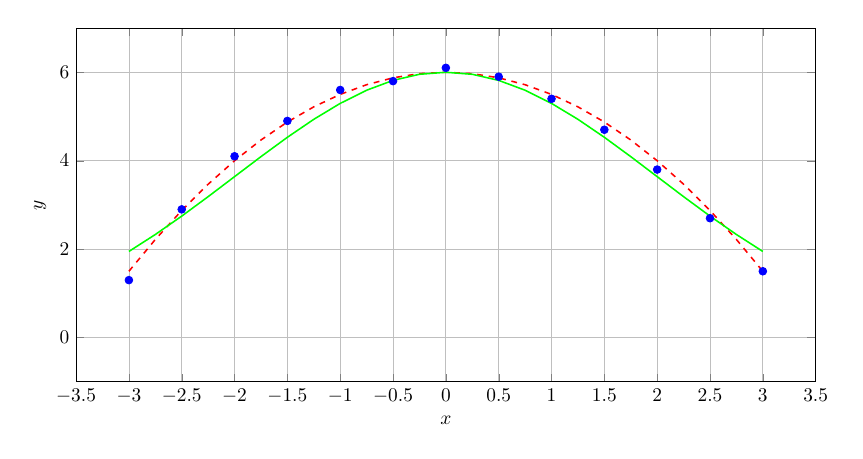
\begin{tikzpicture}[scale=0.7]
      \begin{axis}[ xlabel={$x$}, ylabel={$y$}, grid=major, width=15cm, height=8cm, domain=-3:3, xmin=-3.5, xmax=3.5, ymin=-1, ymax=7 ]

      % Plot scattered points that roughly follow the quadratic pattern
      \addplot[only marks, mark=*, mark size=2pt, blue] coordinates {
        (-3, 1.3)
        (-2.5, 2.9)
        (-2, 4.1)
        (-1.5, 4.9)
        (-1, 5.6)
        (-0.5, 5.8)
        (0, 6.1)
        (0.5, 5.9)
        (1, 5.4)
        (1.5, 4.7)
        (2, 3.8)
        (2.5, 2.7)
        (3, 1.5)
      };
     
      % The quadratic curve
      \addplot[red, thick, dashed] {6 - 0.5*x^2};
     
      % Gaussian-looking curve
      \addplot[green, thick] {6*exp(-x^2/8)};
     
      \end{axis}
    \end{tikzpicture}
    \caption{Diagram of the boundary bias. The green line represents what you would see for a fitted kernel regressor. At the boundaries (endpoints of the data), you can see that because the kernel is cut off, more and more bias accumulates. We avoid this in local polynomial regression.} 
  \end{figure}

\subsection{Local Polynomial Regression}

  We can extend this and compute local polynomials rather than lines. 

  \begin{definition}[Local Polynomial Estimator]
    The \textbf{local polynomial estimator} is a local linear kernel smoother that estimates the function $\hat{f}$ that minimizes the following loss. 
    \begin{equation}
      \argmin_{\beta} \sum_i K \bigg( \frac{X_i - x}{h} \bigg) \big( Y_i - (\beta_0 (x) - \beta_1 (x) (x- X_i) + \ldots + \beta_k (x) (x - X_i)^k )\big)
    \end{equation}
  \end{definition}

  People do this because there is also bias in the peaks and troughs of the data, and local quadratics can capture this much better. Beyond quadratics, there's not much more benefits and we have the accumulating cost of variance. 

\section{Splines}

  This is not local, but it's a linear smoother. 


\section{RKHS Regression}

  This is not local, but it's a linear smoother. 


\section{Additive Models and Naive Bayes}

  Additive models and naive bayes are both nonparameteric methods, but they are very similar. 

\subsection{Additive Models}

  In the most general case, we want to create nonparametric regression functions of the form 
  \begin{equation}
    Y = f(x_1, \ldots, x_d) + \epsilon 
  \end{equation}
  We've done this for one dimensional case, but we can extend this to multiple dimensions through additive models of the form 
  \begin{equation}
    Y = \sum_j f_j (x_j)  + \epsilon
  \end{equation}
  This gives us very interpretable models where we can clearly see the effect of each covariate on $Y$. Clearly, this is not as flexible as the previous model since they can't capture dependencies, but we can create sub-dependency functions and replace the form above to something like 
  \begin{equation}
    Y = \sum_{i, j} f_{i, j} (x_i, x_j) + \epsilon
  \end{equation}
  giving us more flexible models. 

\subsection{Naive Bayes} 

  Say we are doing a binary classification problem. We treat the features as independent (which is very unrealistic) and model the probability distribution as 
  \begin{equation}
    p(x \mid y = 0) = \prod_{j=1}^d p_j (x_j \mid y = 0), \qquad p(x \mid y = 1) = \prod_{j=1}^d p_j (x_j \mid y = 1)
  \end{equation}

  When we take the log, we can see that it is like the additive model. This turns out to be surprisingly successful. 

\section{Nonlinear Smoothers, Trend Filtering} 

  Tough example of the Dobbler function (like topologists sine curve). It's a pretty good fit but it's not too good since it's using a linear smoother (homogeneous). So we might need to fit it with nonlinear smoothers. 


\section{Support Vector Machines} 

  Remember that it was the assumption that the conditional distribution $Y \mid X = x$ being Bernoulli/multinomial, along with the power form of the surrogate likelihood, that led to the likelihood derivation of the surrogate loss of the logistic and softmax regression. But ultimately, these are just modeling assumptions, and we may look for other surrogate losses to construct our risk. 

  If we want to construct such a loss function, we first want it to approximate the $0$-$1$ step function clearly. The next thing is that we want it to be convex, so we can use convex optimization (sum of convex functions are convex). Perhaps we can think of the \textit{smallest} convex function that stays above the binary loss, in some sense the best approximation. This is precisely the hinge function. 

  \begin{definition}[Hinge Loss]
    The \textbf{hinge loss} is a convex surrogate loss function for the 0-1 loss function. It is defined as 
    \begin{equation}
      L(y, \hat{y}) = \max(0, 1 - y \cdot \hat{y})
    \end{equation}
  \end{definition} 

  Note that we have directly constructed a loss without any reference to the likelihood of the data points. Now the SVM model is really simple. We just have a linear model $g(x) = \beta^T x$, and then use it to make a plug-in classifier through a threshold function with threshold $0$. 

  \begin{definition}[Binary Support Vector Machine]
    The \textbf{binary SVM} is a linear classifier that sets 
    \begin{equation}
      f(x) = \mathrm{sign}(F(x)) = \mathrm{sign}(\beta^T x) = \begin{cases} 
        1 & \text{ if } \beta^T x \geq 0 \\
        0 & \text{ else}
      \end{cases}
    \end{equation}
  \end{definition} 

  With the model and loss set up, we can define our risk.

  \begin{theorem}[Risk]
    The expected risk is 
    \begin{equation}
      R(f) = \mathbb{E}_{x, y} \left[ \max\{0, 1 - y F(x) \}\right] = \mathbb{E}_{x, y} \left[ \max\{0, 1 - y (\beta^T x) \}\right]
    \end{equation}
    and the empirical risk is 
    \begin{equation}
      \hat{R}(f) = \frac{1}{n} \sum_{i=1}^n \max\{0, 1 - y (\beta^T x) \}
    \end{equation}
  \end{theorem}
  
  Note that if we classified something correctly, then $y(\beta^T x)$ would be positive, leading to the loss term being cut off to $0$.\footnote{Unless $\beta^T x$ was a very small positive number, but speaking loosely here.} So the model will focus only on the points that are wrong or that are most difficult to tell apart. This is a big difference between SVMs and other classifiers. 

  \begin{example}[SVMs vs Other Classifiers on Linearly Separable Dataset]
    Assume that our dataset $\mathcal{D} = \{\mathbf{x}_i, y_i\}$ is linearly separable with $y_i \in \{-1, +1\}$. Based on previous algorithms like the perceptron, it will find some separating hyperplane. However, there's an infinite number of separating hyperplanes as shown in Figure \ref{fig:svm_intro_1}. What support vector machines want to do is to find the best one, with the ``best" defined as the hyperplane that maximizes the distance between either the closest positive or negative samples, shown in Figure $\ref{fig:svm_intro2}$.  

    \begin{figure}[H] 
      \centering 
      \begin{subfigure}[b]{0.45\textwidth} 
        \centering 
        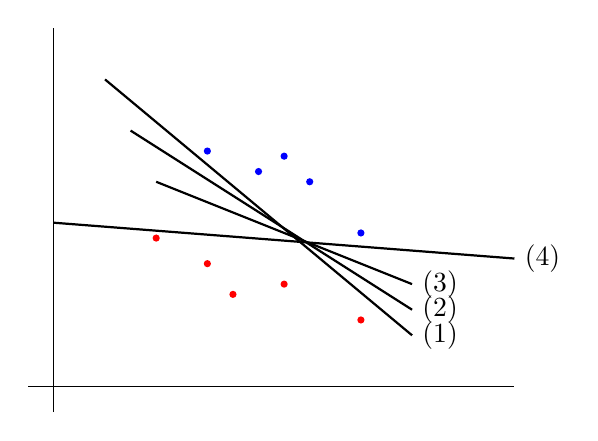
\begin{tikzpicture}[scale=0.65]
          % Draw axes
          \draw[-] (-0.5,0) -- (9,0);
          \draw[-] (0,-0.5) -- (0,7);
          
          % Intersection point
          \coordinate (I) at (4,3);
          
          % Draw numbered lines
          \draw[thick] (1,6) -- (7,1) node[right] {(1)};
          \draw[thick] (1.5,5) -- (7,1.5) node[right] {(2)};
          \draw[thick] (2,4) -- (7,2) node[right] {(3)};
          \draw[thick] (0,3.2) -- (9,2.5) node[right] {(4)};
          
          % Add blue points (above lines)
          \fill[blue] (3,4.6) circle (2pt);
          \fill[blue] (4,4.2) circle (2pt);
          \fill[blue] (5,4) circle (2pt);
          \fill[blue] (6,3) circle (2pt);
          \fill[blue] (4.5,4.5) circle (2pt);
          
          % Add red points (below lines)
          \fill[red] (2,2.9) circle (2pt);
          \fill[red] (3,2.4) circle (2pt);
          \fill[red] (3.5,1.8) circle (2pt);
          \fill[red] (4.5,2) circle (2pt);
          \fill[red] (6,1.3) circle (2pt);
        \end{tikzpicture}
        \caption{Planes such as (1) and (4) are ``too close" to the positive and negative samples. } 
        \label{fig:svm_intro_1}
      \end{subfigure}
      \hfill
      \begin{subfigure}[b]{0.45\textwidth} 
        \centering 
        \begin{tikzpicture}[scale=0.65]
          % Draw axes
          \draw[-] (-0.5,0) -- (9,0);
          \draw[-] (0,-0.5) -- (0,7);
          
          % Intersection point
          \coordinate (I) at (4,3);
          
          % Draw numbered lines
          \draw[thick] (1,5) -- (7,1.5);
          \draw[dotted, thick] (1,5.8) -- (7,2.3);
          \draw[dotted, thick] (1,4.2) -- (7,0.7);
          
          % Add blue points (above lines)
          \fill[blue] (3,4.6) circle (2pt);
          \fill[blue] (4,4.2) circle (2pt);
          \fill[blue] (5,4) circle (2pt);
          \fill[blue] (6,3) circle (2pt);
          \fill[blue] (4.5,4.5) circle (2pt);
          
          % Add red points (below lines)
          \fill[red] (2,2.9) circle (2pt);
          \fill[red] (3,2.4) circle (2pt);
          \fill[red] (3.5,1.8) circle (2pt);
          \fill[red] (4.5,2) circle (2pt);
          \fill[red] (6,1.3) circle (2pt);
        \end{tikzpicture}
        \caption{SVMs try to find the separating hyperplane with the best minimum margin.} 
        \label{fig:svm_intro2}
      \end{subfigure} 
      \caption{Motivating problem} 
      \label{fig:svm_intro} 
    \end{figure}
  \end{example} 

  We want to formalize the concepts of these margins that we wish to maximize. Furthermore, this problem is not well defined since we can just set $w$ to be $0$ or an arbitrarily high norm vector, which makes this problem ill-posed. Therefore, we will need some constraints as well. 

\subsection{Functional and Geometric Margins} 
  
  To do this, we will define two terms. 

  \begin{definition}[Geometric margin]
    Given a point $\mathbf{x}_0$ and a hyperplane of equation $\mathbf{w} \cdot \mathbf{x} + b = 0$, the distance from $\mathbf{x}_0$ to the hyperplane, known as the \textbf{geometric margin}, can be computed with the formula 

    \begin{equation}
      d = \frac{|\mathbf{x}_0 \cdot \mathbf{w} + b|}{||\mathbf{w}||}  
    \end{equation} 

    Therefore, the geometric margin of the $i$th sample with respect to the hypothesis $f$ is defined 

    \begin{equation}
      \gamma_i = \frac{y_i \, (\mathbf{w} \cdot \mathbf{x}_i + b)}{||\mathbf{w}||} 
    \end{equation} 
  \end{definition}

  We wish to optimize the parameters $\mathbf{w}, b$ in order to maximize the minimum of the geometric margins (the distance between the closest point and the hyperplane). 

  \begin{equation}
    \argmax_{\mathbf{w}, b} \min_i \gamma_i = \argmax_{\mathbf{w}, b} \bigg\{ \frac{1}{||\mathbf{w}||} \min_i \big[y_i \, (\mathbf{w} \cdot \mathbf{x}_i + b) \big] \bigg\}
  \end{equation}

  Direct solution of this optimization problem would be very complex, and so we convert this into an equivalent problem that is much easier to solve. Note that the solution to the above term is not unique. If there was a solution $(\mathbf{w}^\ast, b^\ast)$, then 

  \begin{equation}
    \frac{y_i (\mathbf{w} \cdot \mathbf{x}_i + b)}{||\mathbf{w}||} = \frac{y_i (\lambda \mathbf{w} \cdot \mathbf{x}_i + \lambda b)}{||\lambda \mathbf{w}||}  
  \end{equation}

  That is, the geometric margin is not sensitive to scaling of the parameters of the hyperplane. Therefore, we can scale the numerator and the denominator by whatever we want and use this freedom to set 

  \begin{equation*}
    y_i ( \mathbf{w} \cdot \mathbf{x}_i + b ) = 1 
  \end{equation*}
  
  for the point that is closest to the surface. In that case, all data points will satisfy the constraints 

  \begin{equation*}
    y_n (\mathbf{w} \cdot \mathbf{x}_i + b) \geq 1
  \end{equation*}

  In the case of data points for which the equality holds, the constraints are said to be \textit{active}, whereas for the remainder they are \textit{inactive}. Therefore, it will always be the case that $\min_i \big[ y_i \, (\mathbf{w} \cdot \mathbf{x}_i + b)\big] = 1$, and the constraint problem reduces to 

  \begin{equation}
    \argmax_{\mathbf{w}, b} \frac{1}{||\mathbf{w}||} = \argmin_{\mathbf{w}, b} \frac{1}{2} ||\mathbf{w}||^2 \text{ subject to constraints } y_i (\mathbf{w} \cdot \mathbf{x}_i + b) \geq 1 
  \end{equation}

  This final step is the most significant step in this derivation and may be hard to wrap around the first time. So we dedicate the next subsubsection for this. 

  
  We could just work straight with this geometric margin, but for now, let's try to extend what we did with the perceptron into SVMs. We will find out that extending the concept of functional margins into SVMs leads to ill-defined problems. In the perceptron, we wanted to construct a function $f(\mathbf{x}) = \mathbf{w} \cdot \mathbf{x} + b$ such that 
  \begin{equation*}
    y_i \, f(\mathbf{x}_i) \geq 0 \text{ for all } i = 1, 2, \ldots, N
  \end{equation*}

  \begin{definition}[Functional Margin]
    The value of $y_i \, f(\mathbf{x}_i)$ gives us our confidence on our classification, and in a way it represents a kind of distance away from the separating hyperplane (if this value was $0$, then we would be 50 50 split on whether to label it positive or negative). Therefore, we shall define 
    \begin{equation*}
        \hat{\gamma}_i = y_i f(\mathbf{x}_i) 
    \end{equation*}
  as the \textbf{functional margin} of $(\mathbf{w}, b)$ with respect to the training sample $(\mathbf{x}_i, y_i)$. Therefore, the smallest of the function margins can be written 
  \begin{equation*}
      \hat{\gamma} = \min_i \gamma_i 
  \end{equation*}
  called the \textbf{function margin}. 
  \end{definition}

  Note that the geometric margin and functional margin are related by a constant scaling factor. Given a sample $(\mathbf{x}_i, y_i)$, we have 
  \begin{equation*}
      \mathrm{Geometric Margin} = \frac{y_i \, (\mathbf{w} \cdot \mathbf{x}_i + b)}{||\mathbf{w}||_2} = \frac{\mathrm{Functional Margin}}{||\mathbf{w}||_2}
  \end{equation*}

  As we can see, the perceptron works with the functional margin, and since it does not care about how large the margin is (just whether it's positive or negative), we are left with an underdetermined system in which there exists infinite $(\mathbf{w}, b)$'s. Now what we want to do is impose a certain minimum margin $\gamma > 0$ and solve for $(\mathbf{w}, b)$ again, and keep increasing this $\gamma$ until there is some unique solution. We can view this problem in two ways: 
  \begin{enumerate} 
      \item Take a specific minimum margin $\gamma$ and find a $(\mathbf{w}, b)$, which may not exist, be unique, or exist infinitely that satisfies 
          \begin{equation*}
              y_i f(\mathbf{x}) = y_i ( \mathbf{w} \cdot \mathbf{x} + b) \geq \gamma \text{ for all } i = 1, \ldots, N 
          \end{equation*}
      \item Take a specific $(\mathbf{w}, b)$ and calculate the maximum $\gamma$ that satisfies the constraint equations above.  
  \end{enumerate}

  They're both equivalent problems, but both ill-posed if we look at (2). Since the samples are linearly separable by assumption, we can say that there exists some $\epsilon > 0$ such that $y_i f(\mathbf{x}_i) \geq \epsilon$ for all $i$. Therefore, if we just scale $(\mathbf{w}, b) \mapsto (\lambda \mathbf{w}, \lambda b)$ for some large $\lambda$, this leads to the solution for $\gamma$ being unbounded. We can see in Figure $\ref{fig:scaling_problem}$ that we can increased confidence at no cost. Looking at (1), we can also see that if $(\mathbf{w}, b)$ does exist, then every other $(\lambda \mathbf{w}, \lambda b)$ for $\lambda > 1$ satisfies the property.   

  \begin{figure}[H] 
    \centering 
    \begin{subfigure}[b]{0.32\textwidth} 
      \centering 
      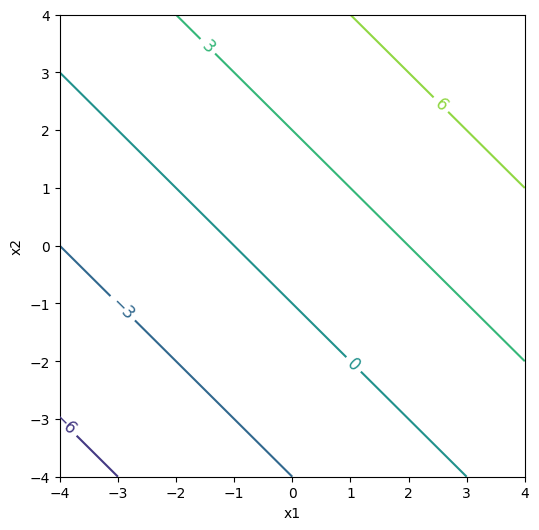
\includegraphics[width=\textwidth]{img/scaling1.png} 
      \caption{$f(x) = x_1 + x_2 + 1$} 
      \label{fig:original_scaled}
    \end{subfigure} 
    \hfill    
    \begin{subfigure}[b]{0.32\textwidth} 
      \centering 
      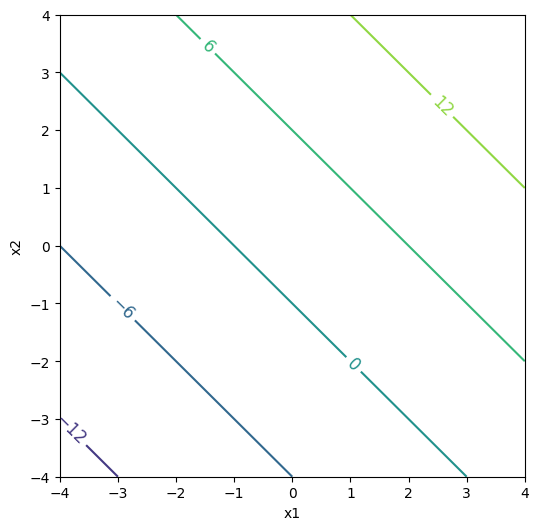
\includegraphics[width=\textwidth]{img/scaling2.png} 
      \caption{$f(x) = 2 x_1 + 2 x_2 + 2$} 
      \label{fig:two_times_scaled}
    \end{subfigure} 
    \hfill
    \begin{subfigure}[b]{0.32\textwidth} 
      \centering 
      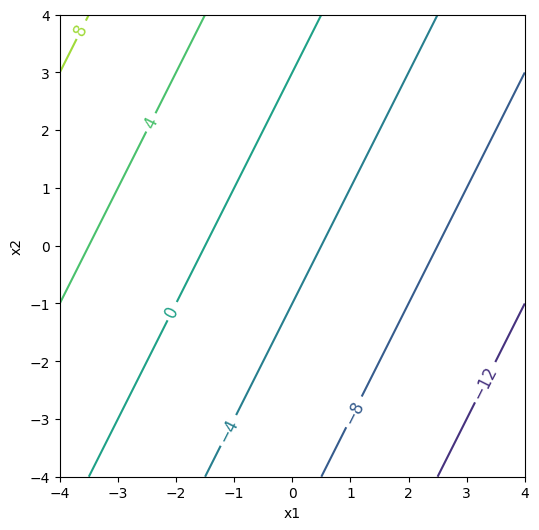
\includegraphics[width=\textwidth]{img/scaling3.png} 
      \caption{$f(x) = -2x_1 + x_2 - 3$} 
      \label{fig:something_else}
    \end{subfigure} 
    \caption{From (a), you can see that simply multiplying everything by two automatically increases our confidence by $2$, meaning that the functional margin can be scaled arbitrarily by scaing $(\mathbf{w}, b)$. There are still too many degrees of freedom in here and so extra constraints must be imposed. } 
    \label{fig:scaling_problem} 
  \end{figure}

\subsection{Analytical Solution} 

  To minimize the equations with the constraint equations, we can use the method of Lagrange multipliers, which leads to to Lagrangian 
  \[\mathcal{L}(\mathbf{w}, b, \boldsymbol{\alpha}) = \frac{1}{2} ||\mathbf{w}||^2 - \sum_i \alpha_i \big[ y_i (\mathbf{w} \cdot \mathbf{x}_i + b) - 1\big]\]
  We can take the gradients with respect to $\mathbf{w}$ and $b$ and set them to $0$, which gives the two conditions 
  \begin{align*} 
    \mathbf{w} & = \sum_i \alpha_i y_i \mathbf{x}_i \\
    0 & = \sum_i \alpha_i y_i \mathbf{x}_i 
  \end{align*}

  Now let's substitute our evaluated $\mathbf{w}$ back into $\mathcal{L}$, which gives the \textbf{dual representation} of the maximum margin problem in which we maximize  
  \begin{align*} 
      L & = \frac{1}{2} \bigg( \sum_i \alpha_i y_i \mathbf{x}_i \bigg) \bigg( \sum_j \alpha_j y_j \mathbf{x}_j \bigg) - \sum_{i} \alpha_i y_i x_i \cdot \bigg[ \sum_j \alpha_j y_j x_j \bigg] - \sum_i \alpha_i y_i b + \sum_i \alpha_i \\ 
        & = \sum_i \alpha_i - \frac{1}{2} \sum_{i, j} \alpha_i \alpha_j y_i y_j \, \mathbf{x}_i \cdot \mathbf{x}_j 
  \end{align*}
  The summation with the $b$ in it is $0$ since we can pull the $b$ out and the remaining sum is $0$ from before. Now the optimization only depends on the dot product $\mathbf{x}_i \cdot \mathbf{x}_j$ of all pairs of sample vectors, which is very interesting. We will see more of this when we talk about kernel methods. Now, we need to solve the dual problem 
  \[\max_{\boldsymbol{\alpha}} \mathcal{L}(\boldsymbol{\alpha})\]
  which can be done using some generic quadratic programming solver or some other method to get the optimum $\boldsymbol{\alpha}^\ast$, which gives us 
  \[\mathbf{w}^\ast = \sum_i \alpha_i^\ast y_i \mathbf{x}_i\]

\subsection{Significance Tests and Confidence Sets}

\subsection{Concentration Bounds} 

\subsection{Nonseparable Case} 



\bibliography{./bibfile}
\bibliographystyle{alpha}
\end{document}
